\documentclass[twoside]{book}

% Packages required by doxygen
\usepackage{fixltx2e}
\usepackage{calc}
\usepackage{doxygen}
\usepackage[export]{adjustbox} % also loads graphicx
\usepackage{graphicx}
\usepackage[utf8]{inputenc}
\usepackage{makeidx}
\usepackage{multicol}
\usepackage{multirow}
\PassOptionsToPackage{warn}{textcomp}
\usepackage{textcomp}
\usepackage[nointegrals]{wasysym}
\usepackage[table]{xcolor}

% Font selection
\usepackage[T1]{fontenc}
\usepackage[scaled=.90]{helvet}
\usepackage{courier}
\usepackage{amssymb}
\usepackage{sectsty}
\renewcommand{\familydefault}{\sfdefault}
\allsectionsfont{%
  \fontseries{bc}\selectfont%
  \color{darkgray}%
}
\renewcommand{\DoxyLabelFont}{%
  \fontseries{bc}\selectfont%
  \color{darkgray}%
}
\newcommand{\+}{\discretionary{\mbox{\scriptsize$\hookleftarrow$}}{}{}}

% Page & text layout
\usepackage{geometry}
\geometry{%
  a4paper,%
  top=2.5cm,%
  bottom=2.5cm,%
  left=2.5cm,%
  right=2.5cm%
}
\tolerance=750
\hfuzz=15pt
\hbadness=750
\setlength{\emergencystretch}{15pt}
\setlength{\parindent}{0cm}
\setlength{\parskip}{3ex plus 2ex minus 2ex}
\makeatletter
\renewcommand{\paragraph}{%
  \@startsection{paragraph}{4}{0ex}{-1.0ex}{1.0ex}{%
    \normalfont\normalsize\bfseries\SS@parafont%
  }%
}
\renewcommand{\subparagraph}{%
  \@startsection{subparagraph}{5}{0ex}{-1.0ex}{1.0ex}{%
    \normalfont\normalsize\bfseries\SS@subparafont%
  }%
}
\makeatother

% Headers & footers
\usepackage{fancyhdr}
\pagestyle{fancyplain}
\fancyhead[LE]{\fancyplain{}{\bfseries\thepage}}
\fancyhead[CE]{\fancyplain{}{}}
\fancyhead[RE]{\fancyplain{}{\bfseries\leftmark}}
\fancyhead[LO]{\fancyplain{}{\bfseries\rightmark}}
\fancyhead[CO]{\fancyplain{}{}}
\fancyhead[RO]{\fancyplain{}{\bfseries\thepage}}
\fancyfoot[LE]{\fancyplain{}{}}
\fancyfoot[CE]{\fancyplain{}{}}
\fancyfoot[RE]{\fancyplain{}{\bfseries\scriptsize Generated by Doxygen }}
\fancyfoot[LO]{\fancyplain{}{\bfseries\scriptsize Generated by Doxygen }}
\fancyfoot[CO]{\fancyplain{}{}}
\fancyfoot[RO]{\fancyplain{}{}}
\renewcommand{\footrulewidth}{0.4pt}
\renewcommand{\chaptermark}[1]{%
  \markboth{#1}{}%
}
\renewcommand{\sectionmark}[1]{%
  \markright{\thesection\ #1}%
}

% Indices & bibliography
\usepackage{natbib}
\usepackage[titles]{tocloft}
\setcounter{tocdepth}{3}
\setcounter{secnumdepth}{5}
\makeindex

% Hyperlinks (required, but should be loaded last)
\usepackage{ifpdf}
\ifpdf
  \usepackage[pdftex,pagebackref=true]{hyperref}
\else
  \usepackage[ps2pdf,pagebackref=true]{hyperref}
\fi
\hypersetup{%
  colorlinks=true,%
  linkcolor=blue,%
  citecolor=blue,%
  unicode%
}

% Custom commands
\newcommand{\clearemptydoublepage}{%
  \newpage{\pagestyle{empty}\cleardoublepage}%
}

\usepackage{caption}
\captionsetup{labelsep=space,justification=centering,font={bf},singlelinecheck=off,skip=4pt,position=top}

%===== C O N T E N T S =====

\begin{document}

% Titlepage & ToC
\hypersetup{pageanchor=false,
             bookmarksnumbered=true,
             pdfencoding=unicode
            }
\pagenumbering{alph}
\begin{titlepage}
\vspace*{7cm}
\begin{center}%
{\Large Decentralized Dummy \\[1ex]\large 1 }\\
\vspace*{1cm}
{\large Generated by Doxygen 1.8.13}\\
\end{center}
\end{titlepage}
\clearemptydoublepage
\pagenumbering{roman}
\tableofcontents
\clearemptydoublepage
\pagenumbering{arabic}
\hypersetup{pageanchor=true}

%--- Begin generated contents ---
\chapter{File Index}
\section{File List}
Here is a list of all files with brief descriptions\+:\begin{DoxyCompactList}
\item\contentsline{section}{/home/visxim/\+C\+Lion\+Projects/\+Decentralized\+Dummy\+Process/\hyperlink{file_8cpp}{file.\+cpp} }{\pageref{file_8cpp}}{}
\item\contentsline{section}{/home/visxim/\+C\+Lion\+Projects/\+Decentralized\+Dummy\+Process/\hyperlink{JSON__manager_8cpp}{J\+S\+O\+N\+\_\+manager.\+cpp} \\*J\+S\+O\+N\+\_\+manager for handling J\+S\+ON data }{\pageref{JSON__manager_8cpp}}{}
\item\contentsline{section}{/home/visxim/\+C\+Lion\+Projects/\+Decentralized\+Dummy\+Process/\hyperlink{main_8cpp}{main.\+cpp} \\*Main of the decentralized dummy process }{\pageref{main_8cpp}}{}
\item\contentsline{section}{/home/visxim/\+C\+Lion\+Projects/\+Decentralized\+Dummy\+Process/\hyperlink{time-tp_8c}{time-\/tp.\+c} }{\pageref{time-tp_8c}}{}
\end{DoxyCompactList}

\chapter{File Documentation}
\hypertarget{file_8cpp}{}\section{/home/visxim/\+C\+Lion\+Projects/\+Decentralized\+Dummy\+Process/file.cpp File Reference}
\label{file_8cpp}\index{/home/visxim/\+C\+Lion\+Projects/\+Decentralized\+Dummy\+Process/file.\+cpp@{/home/visxim/\+C\+Lion\+Projects/\+Decentralized\+Dummy\+Process/file.\+cpp}}
{\ttfamily \#include \char`\"{}file.\+h\char`\"{}}\newline
Include dependency graph for file.\+cpp\+:
\nopagebreak
\begin{figure}[H]
\begin{center}
\leavevmode
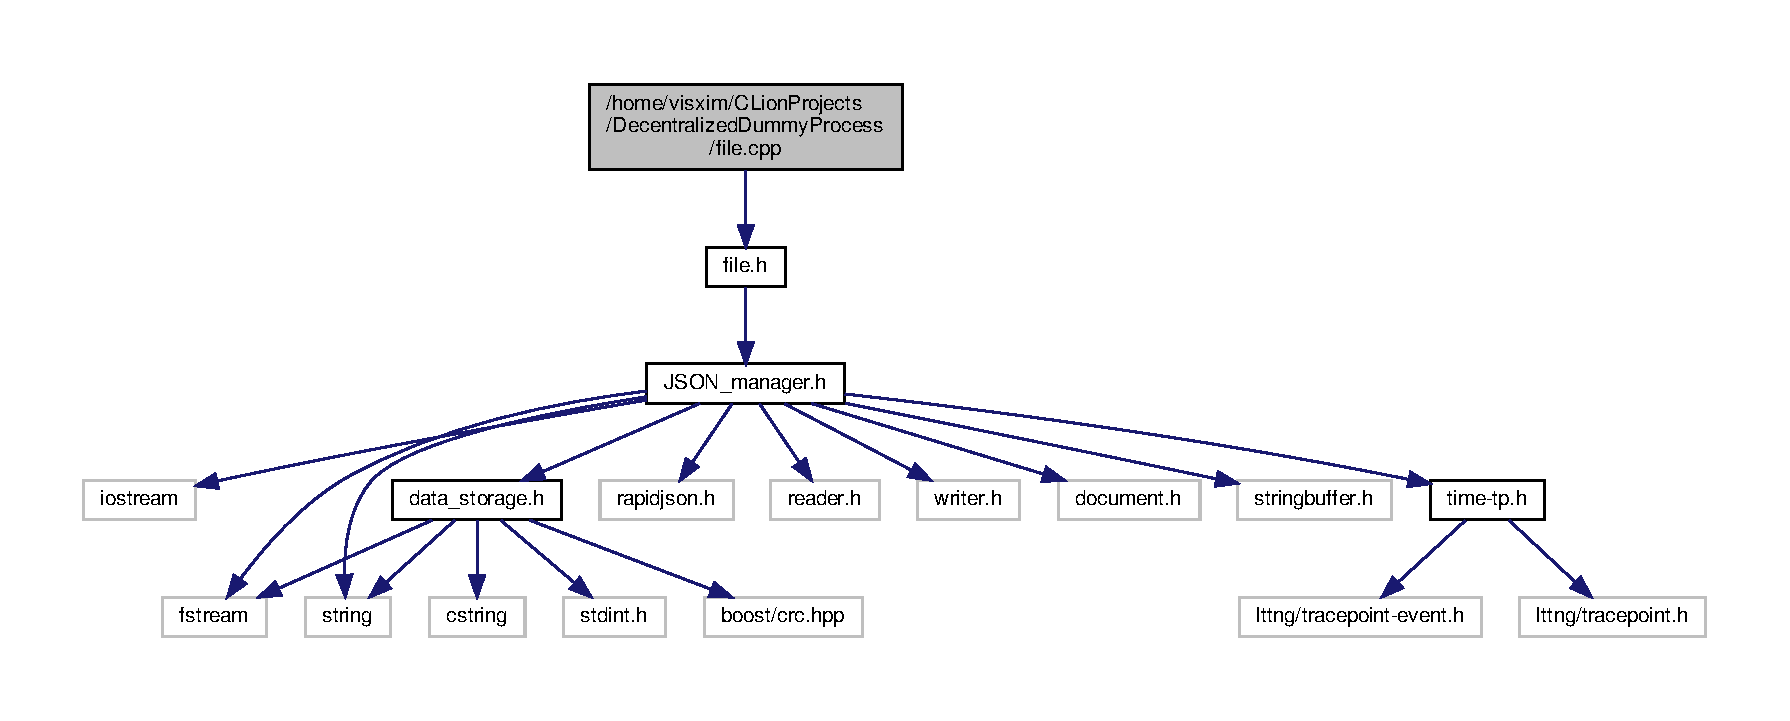
\includegraphics[width=350pt]{file_8cpp__incl}
\end{center}
\end{figure}

\hypertarget{JSON__manager_8cpp}{}\section{/home/visxim/\+C\+Lion\+Projects/\+Decentralized\+Dummy\+Process/\+J\+S\+O\+N\+\_\+manager.cpp File Reference}
\label{JSON__manager_8cpp}\index{/home/visxim/\+C\+Lion\+Projects/\+Decentralized\+Dummy\+Process/\+J\+S\+O\+N\+\_\+manager.\+cpp@{/home/visxim/\+C\+Lion\+Projects/\+Decentralized\+Dummy\+Process/\+J\+S\+O\+N\+\_\+manager.\+cpp}}


J\+S\+O\+N\+\_\+manager for handling J\+S\+ON data.  


{\ttfamily \#include \char`\"{}J\+S\+O\+N\+\_\+manager.\+h\char`\"{}}\newline
Include dependency graph for J\+S\+O\+N\+\_\+manager.\+cpp\+:
\nopagebreak
\begin{figure}[H]
\begin{center}
\leavevmode
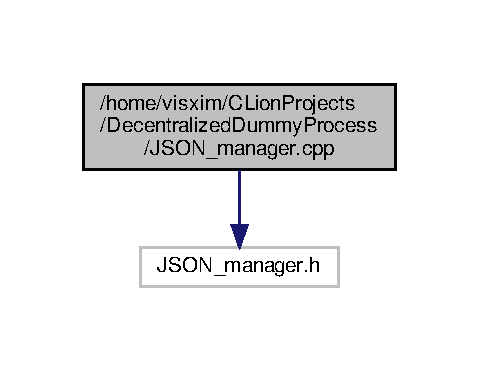
\includegraphics[width=230pt]{JSON__manager_8cpp__incl}
\end{center}
\end{figure}


\subsection{Detailed Description}
J\+S\+O\+N\+\_\+manager for handling J\+S\+ON data. 

The J\+S\+O\+N\+\_\+manager handels the interpretation and storage of the J\+S\+ON data from the given file 
\hypertarget{main_8cpp}{}\section{/home/visxim/\+C\+Lion\+Projects/\+Decentralized\+Dummy\+Process/main.cpp File Reference}
\label{main_8cpp}\index{/home/visxim/\+C\+Lion\+Projects/\+Decentralized\+Dummy\+Process/main.\+cpp@{/home/visxim/\+C\+Lion\+Projects/\+Decentralized\+Dummy\+Process/main.\+cpp}}


main of the decentralized dummy process  


{\ttfamily \#include \char`\"{}file.\+h\char`\"{}}\newline
{\ttfamily \#include \char`\"{}time-\/tp.\+h\char`\"{}}\newline
Include dependency graph for main.\+cpp\+:
\nopagebreak
\begin{figure}[H]
\begin{center}
\leavevmode
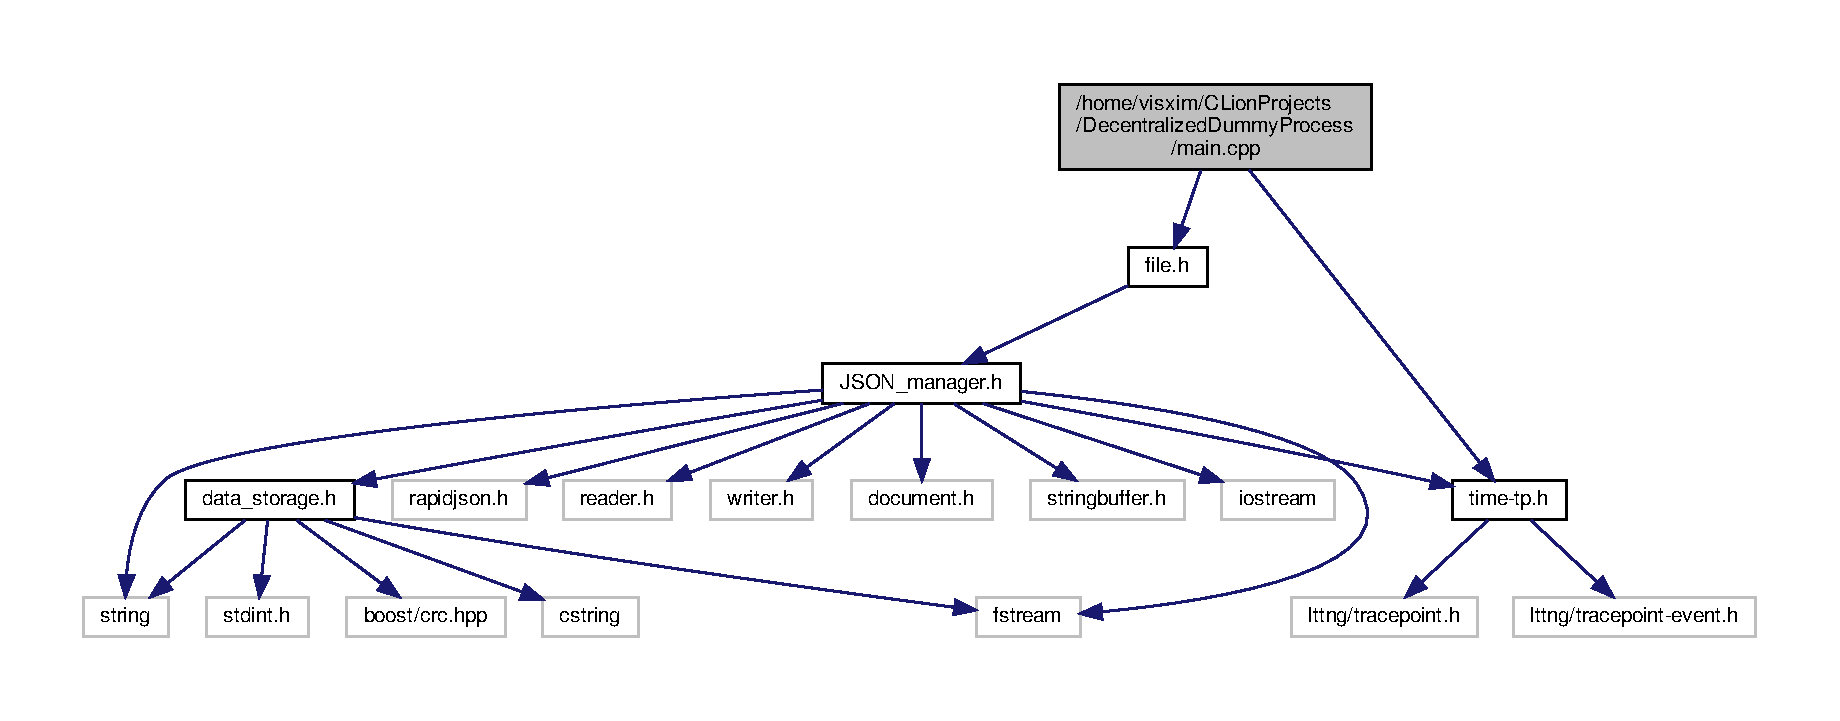
\includegraphics[width=350pt]{main_8cpp__incl}
\end{center}
\end{figure}
\subsection*{Functions}
\begin{DoxyCompactItemize}
\item 
int \hyperlink{main_8cpp_a3c04138a5bfe5d72780bb7e82a18e627}{main} (int argc, char $\ast$$\ast$argv)
\begin{DoxyCompactList}\small\item\em main function \end{DoxyCompactList}\end{DoxyCompactItemize}


\subsection{Detailed Description}
main of the decentralized dummy process 



\subsection{Function Documentation}
\mbox{\Hypertarget{main_8cpp_a3c04138a5bfe5d72780bb7e82a18e627}\label{main_8cpp_a3c04138a5bfe5d72780bb7e82a18e627}} 
\index{main.\+cpp@{main.\+cpp}!main@{main}}
\index{main@{main}!main.\+cpp@{main.\+cpp}}
\subsubsection{\texorpdfstring{main()}{main()}}
{\footnotesize\ttfamily int main (\begin{DoxyParamCaption}\item[{int}]{argc,  }\item[{char $\ast$$\ast$}]{argv }\end{DoxyParamCaption})}



main function 

Here is the call graph for this function\+:
\nopagebreak
\begin{figure}[H]
\begin{center}
\leavevmode
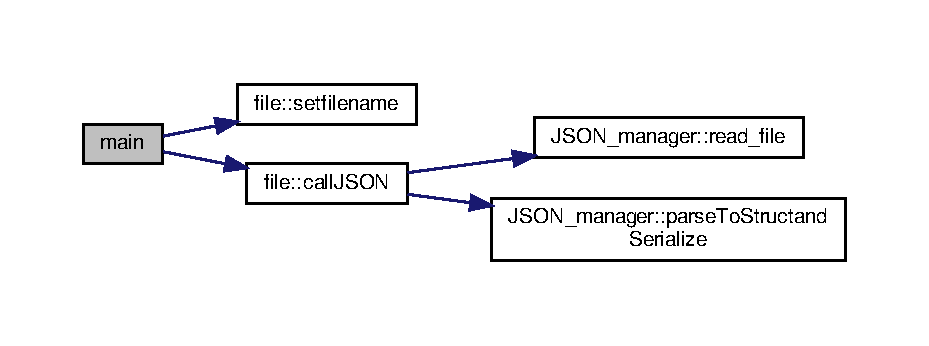
\includegraphics[width=350pt]{main_8cpp_a3c04138a5bfe5d72780bb7e82a18e627_cgraph}
\end{center}
\end{figure}

\hypertarget{time-tp_8c}{}\section{/home/visxim/\+C\+Lion\+Projects/\+Decentralized\+Dummy\+Process/time-\/tp.c File Reference}
\label{time-tp_8c}\index{/home/visxim/\+C\+Lion\+Projects/\+Decentralized\+Dummy\+Process/time-\/tp.\+c@{/home/visxim/\+C\+Lion\+Projects/\+Decentralized\+Dummy\+Process/time-\/tp.\+c}}
{\ttfamily \#include \char`\"{}time-\/tp.\+h\char`\"{}}\newline
Include dependency graph for time-\/tp.c\+:
\nopagebreak
\begin{figure}[H]
\begin{center}
\leavevmode
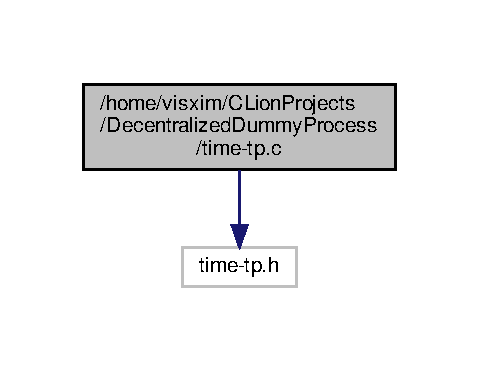
\includegraphics[width=230pt]{time-tp_8c__incl}
\end{center}
\end{figure}
\subsection*{Macros}
\begin{DoxyCompactItemize}
\item 
\#define \hyperlink{time-tp_8c_aeb980b4a64d9b54d660780a30415b0bc}{T\+R\+A\+C\+E\+P\+O\+I\+N\+T\+\_\+\+C\+R\+E\+A\+T\+E\+\_\+\+P\+R\+O\+B\+ES}
\item 
\#define \hyperlink{time-tp_8c_a71ad37c54f22eb10bdfed4267d53bd79}{T\+R\+A\+C\+E\+P\+O\+I\+N\+T\+\_\+\+D\+E\+F\+I\+NE}
\end{DoxyCompactItemize}


\subsection{Macro Definition Documentation}
\mbox{\Hypertarget{time-tp_8c_aeb980b4a64d9b54d660780a30415b0bc}\label{time-tp_8c_aeb980b4a64d9b54d660780a30415b0bc}} 
\index{time-\/tp.\+c@{time-\/tp.\+c}!T\+R\+A\+C\+E\+P\+O\+I\+N\+T\+\_\+\+C\+R\+E\+A\+T\+E\+\_\+\+P\+R\+O\+B\+ES@{T\+R\+A\+C\+E\+P\+O\+I\+N\+T\+\_\+\+C\+R\+E\+A\+T\+E\+\_\+\+P\+R\+O\+B\+ES}}
\index{T\+R\+A\+C\+E\+P\+O\+I\+N\+T\+\_\+\+C\+R\+E\+A\+T\+E\+\_\+\+P\+R\+O\+B\+ES@{T\+R\+A\+C\+E\+P\+O\+I\+N\+T\+\_\+\+C\+R\+E\+A\+T\+E\+\_\+\+P\+R\+O\+B\+ES}!time-\/tp.\+c@{time-\/tp.\+c}}
\subsubsection{\texorpdfstring{T\+R\+A\+C\+E\+P\+O\+I\+N\+T\+\_\+\+C\+R\+E\+A\+T\+E\+\_\+\+P\+R\+O\+B\+ES}{TRACEPOINT\_CREATE\_PROBES}}
{\footnotesize\ttfamily \#define T\+R\+A\+C\+E\+P\+O\+I\+N\+T\+\_\+\+C\+R\+E\+A\+T\+E\+\_\+\+P\+R\+O\+B\+ES}

\mbox{\Hypertarget{time-tp_8c_a71ad37c54f22eb10bdfed4267d53bd79}\label{time-tp_8c_a71ad37c54f22eb10bdfed4267d53bd79}} 
\index{time-\/tp.\+c@{time-\/tp.\+c}!T\+R\+A\+C\+E\+P\+O\+I\+N\+T\+\_\+\+D\+E\+F\+I\+NE@{T\+R\+A\+C\+E\+P\+O\+I\+N\+T\+\_\+\+D\+E\+F\+I\+NE}}
\index{T\+R\+A\+C\+E\+P\+O\+I\+N\+T\+\_\+\+D\+E\+F\+I\+NE@{T\+R\+A\+C\+E\+P\+O\+I\+N\+T\+\_\+\+D\+E\+F\+I\+NE}!time-\/tp.\+c@{time-\/tp.\+c}}
\subsubsection{\texorpdfstring{T\+R\+A\+C\+E\+P\+O\+I\+N\+T\+\_\+\+D\+E\+F\+I\+NE}{TRACEPOINT\_DEFINE}}
{\footnotesize\ttfamily \#define T\+R\+A\+C\+E\+P\+O\+I\+N\+T\+\_\+\+D\+E\+F\+I\+NE}


%--- End generated contents ---

% Index
\backmatter
\newpage
\phantomsection
\clearemptydoublepage
\addcontentsline{toc}{chapter}{Index}
\printindex

\end{document}
